%%%%%%%%%%%%%%%%%%%%%%%%%%%%%%%%%%%%%%%%%%%%%%%%%%%%%%%%%%%%%%%%%%%%%%%%%%%%%%%%%%%%%%%%%%%%%%%%%%%%%%%%%%%%%%%%%%%%%%%%%%%%%%%%%%%%%%%%%%%%%%%%%%%%%%%%%%%%%%%%%%%
% Written By Michael Brodskiy
% Class: Fundamentals of Electronics
% Professor: M. Onabajo
%%%%%%%%%%%%%%%%%%%%%%%%%%%%%%%%%%%%%%%%%%%%%%%%%%%%%%%%%%%%%%%%%%%%%%%%%%%%%%%%%%%%%%%%%%%%%%%%%%%%%%%%%%%%%%%%%%%%%%%%%%%%%%%%%%%%%%%%%%%%%%%%%%%%%%%%%%%%%%%%%%%

\include{Includes.tex}

\title{Lecture 7}
\date{\today}
\author{Michael Brodskiy\\ \small Professor: M. Onabajo}

\begin{document}

\maketitle

\begin{itemize}

  \item Silicon Diodes

    \begin{itemize}

      \item Applications

        \begin{itemize}

          \item Rectifiers (AC-to-DC converters)

          \item Overvoltage protection circuits

          \item Signal processing

        \end{itemize}

      \item Small-signal silicon diodes

        \begin{itemize}

          \item Low and medium power applications

          \item Discrete components (in lab)

        \end{itemize}

      \item Circuit symbol: a triangle (positive side, anode), with a vertical line through the point (negative side, cathode)

        \begin{figure}[H]
          \centering
          \tikzset{every picture/.style={line width=0.75pt}} %set default line width to 0.75pt        

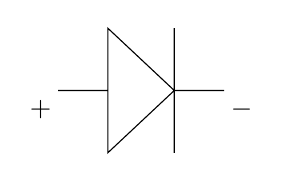
\begin{tikzpicture}[x=0.75pt,y=0.75pt,yscale=-1,xscale=1]
%uncomment if require: \path (0,757); %set diagram left start at 0, and has height of 757

%Shape: Diode [id:dp9916766022166023] 
\draw   (124,108) -- (156,138) -- (124,168) -- (124,108) -- cycle (100,138) -- (124,138) (156,108) -- (156,168) (156,138) -- (180,138) ;

% Text Node
\draw (98,141.4) node [anchor=north east] [inner sep=0.75pt]    {$+$};
% Text Node
\draw (182,141.4) node [anchor=north west][inner sep=0.75pt]    {$-$};


\end{tikzpicture}

          \caption{Diode Symbol}
          \label{fig:1}
        \end{figure}

      \item Diodes dissipate power

    \end{itemize}

  \item Ideal Diode Model

    \begin{itemize}

      \item Rough approximation

        \begin{itemize}

          \item For quick and intuitive circuit analysis

          \item Idealized transfer characteristic (without forward voltage drop and reverse breakdown)

        \end{itemize}

      \item In the reverse bias region, $V<0\to i=0$, while, in the forward bias region, $i>0\to V=0$

    \end{itemize}

  \item Analysis Using the Ideal Diode Model

    \begin{enumerate}

      \item Assume each diode is either open/reverse-biased (RB) or short/forward-biased (FB)

      \item Redraw the circuit while replacing all assumed RB diodes with open-circuits and all FB diodes with short-circuit

      \item Following conventional circuit analysis, solve for:

        \begin{itemize}

          \item Voltages across RB diodes $\to$ verify $V_d<0$

          \item Currents through FB diodes $\to$ verify $i_d>0$

        \end{itemize}

      \item If all assumptions are correct, then the analysis is complete. If any of the RB/FB conditions are not met, proceed with step 1 by making different assumptions for diodes.

    \end{enumerate}

\end{itemize}

\end{document}

